%
% Simple asymmetric two-column CV 
% Author: Sofia JIJON
%

\documentclass[a4paper,10pt]{article}
\usepackage[vmargin=1.5cm, hmargin=1.5cm]{geometry}
% !TEX root = Simple-CV.tex
%-------------------------------------------------------------------------------------------------------
% Packages
%-------------------------------------------------------------------------------------------------------
\usepackage[latin1]{inputenc}
\usepackage[T1]{fontenc}
\usepackage[english]{babel}
\usepackage{fontawesome}
\usepackage{datetime}
\usepackage[usenames,dvipsnames]{xcolor}
\usepackage[colorlinks=true, urlcolor=ColorTwo]{hyperref}
\usepackage{tikz}
\usepackage{hyperref}
\usepackage{setspace}
\usepackage{graphicx}
\usepackage{enumitem}
\usepackage{sectsty}
\usepackage{multicol}
\usepackage{adjustbox}
%-------------------------------------------------------------------------------------------------------
% Layout
%-------------------------------------------------------------------------------------------------------
\pagenumbering{gobble}
\renewcommand{\baselinestretch}{1.5} 
\setlength{\parindent}{0pt}

%
% Color theme
%
\definecolor{ColorOne}{RGB}{0,110,140} 	% Blue
\definecolor{ColorTwo}{RGB}{120,0,120} 	% Mauve
%\definecolor{ColorTwo}{RGB}{140,100,0} 	% Gold

\sectionfont{\color{ColorOne}} 
\subsectionfont{\color{ColorOne}} 

%
% Vertical line
%
\newcommand{\MyVerticalRule}{%
	\textcolor{ColorOne}{\rule{1pt}{\textheight}}
}

%
% Update
%
\newcommand{\LastUpdate}{%
\vfill
\centering \small
\textcolor{ColorOne}{Last updated: \monthname,~\the\year.}
}

%
% Skip
%
\newcommand{\MySkip}{
\vskip12pt
}

%
% Format hyperrefs
%
\newcommand{\myhref}[2]{%
\href{#1}{\textcolor{ColorTwo}{#2}}
}
%
% Format skill bullets
%
\newcommand{\SkillBull}[1]{%
\textcolor{ColorTwo}{#1}
}


%-------------------------------------------------------------------------------------------------------

\begin{document}
\thispagestyle{empty}

%-------------------------------------------------------------------------------------------------------
% Left column
%-------------------------------------------------------------------------------------------------------
\begin{adjustbox}{valign=t}
\begin{minipage}{0.3\textwidth} % Adapt width to your convenience
%----------------------------------------------------
% Please add a photo in 1x1 format
\begin{center}
\begin{tikzpicture}
	\clip (0,0) circle (2cm) node {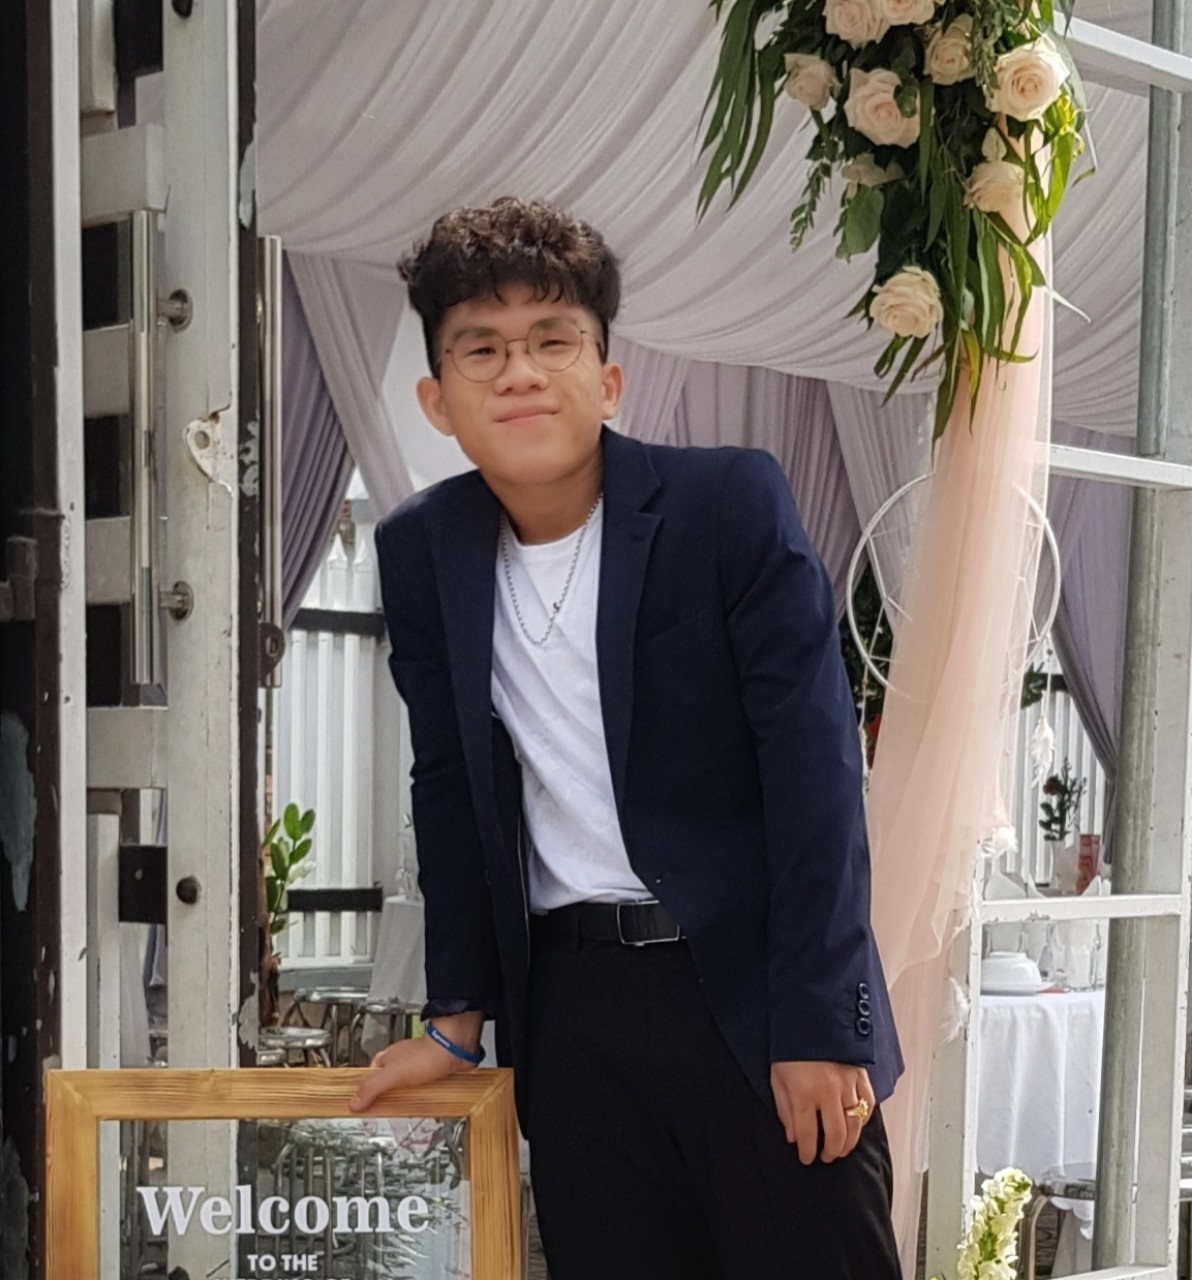
\includegraphics[width=4cm]{./images/avatar.png}};
\end{tikzpicture}

\MySkip 	% See MySetup.tex file

%----------------------------------------------------
{\LARGE \bfseries Manh Cuong Duong}

\MySkip 	% See MySetup.tex file

Born on April 8th, 1999\\
Currently living in Ho Chi Minh City\\

\MySkip 	% See MySetup.tex file

\textcolor{ColorTwo}{\faEnvelopeO} 
\myhref{cuongpigerr@gmail.com}{cuongpigerr@gmail.com} \\

\textcolor{ColorTwo}{\faGithub} 
\myhref{https://github.com/cuongpiger}{https://github.com/cuongpiger}\\

\textcolor{ColorTwo}{\faPhone} 
\myhref{}{+84 0786333545}
\end{center}

\vfill

%----------------------------------------------------
\section*{Scientific interests}
\raggedright
\textcolor{ColorOne}{$\circ$} Data Science\\
\textcolor{ColorOne}{$\circ$} Deep Learning\\
\textcolor{ColorOne}{$\circ$} Machine Learning\\
\textcolor{ColorOne}{$\circ$} Big Data\\

\vfill

%----------------------------------------------------
\section*{Education}
	\begin{description}
	\raggedright
	\item [\normalfont \textcolor{ColorOne}{2022.}] \textbf{Bachelor in Computer Science with} \textcolor{red}{\large\textbf{{GPA 8.4}}}\\ 
	University of Science \\
	District 5, Ho Chi Minh City

	\item [\normalfont \textcolor{ColorOne}{2019.}] \textbf{Getting advanced algorithms certificate}\\
	Big-O Coding Centre\\
	District 3, Ho Chi Minh City

	\item [\normalfont \textcolor{ColorOne}{2018.}] \textbf{Getting basic algorithms certificate}\\
	Big-O Coding Centre\\
	District 3, Ho Chi Minh City
\end{description}

\vfill
\end{minipage}
\end{adjustbox}
%
%
%-------------------------------------------------------------------------------------------------------
% Vertical rule
%-------------------------------------------------------------------------------------------------------
%
\hfill
\begin{adjustbox}{valign=t}
\begin{minipage}{0.05\textwidth} % Adapt width to your convenience
\MyVerticalRule  % See MySetup.tex file
\end{minipage}
\end{adjustbox}
\hfill
%
%-------------------------------------------------------------------------------------------------------
% Right column
%-------------------------------------------------------------------------------------------------------
\begin{adjustbox}{valign=t}
\begin{minipage}{0.6\textwidth} % Adapt width to your convienience
\section*{Skills}
\begin{description}
\raggedright
\item[\normalfont \textcolor{ColorOne}{Data Science, Machine Learning, Deep Learning}] \textbf{}\\ \medskip

\textbf{Programming Languages}: Python, Java, C \& CPP, R, Julia, JavaScript \textit{(for data scraping)}\\
\textbf{Frameworks \& Libraries}: \texttt{TensorFlow}, \texttt{sklearn}, \texttt{keras}, \texttt{numpy}, \texttt{pandas}, \texttt{spark}, \texttt{GraphFrame}, \texttt{opencv}, \texttt{matplotlib}, \texttt{seaborn}, \texttt{plotly}...\\

\item[\normalfont \textcolor{ColorOne}{Database}] \textbf{}\\ \medskip
\textbf{SQL}: MySQL, MS-SQL, PostgreSQL, MariaDB.\\
\textbf{NoSQL}: MongoDB, Firebase.\\

\item[\normalfont \textcolor{ColorOne}{Others}] \textbf{}\\ \medskip
\textbf{Web}: Django, Flask.\\
\textbf{Mobile}: Android Java.\\
\textbf{Desktop App:} PyQT5, PySide2.\\
\textbf{Operation System}: Linux distro Ubuntu 20.04 \textit{(4 years)}.
\textbf{Markup Languages}: HTML, CSS, Markdown, LaTex, Beamer,...\\

\end{description}

%----------------------------------------------------
\section*{Products \& Projects}
\begin{description}
\raggedright
\item[\normalfont \textcolor{ColorOne}{Sentiment Analysis for customers' reviews}] 
\textit{(data scraping from comments in fashion products of Shopee Vietnam)}\\ \medskip
	
	\textbf{Project's link}: \myhref{https://github.com/cuongpiger/SCL_KHVW_Sentiment_Analysis_Project}{github.com/cuongpiger/SCL\_KHVW\_Sentiment\_Analysis\_Project}
	\textbf{Description}: Categorize customers into two groups of positive or negative based on their comments. The model accuracy is 97\% with LSTM.\\

	\textbf{Techniques}: Scraping data, pre-processing text data, visualization, transforming and exploring data, applying traditional machine learning \& deep learning, model evaluation.\\
	
\item[\normalfont \textcolor{ColorOne}{Images generating with DC-GANs}] 
	\textbf{}\\ \medskip

	\textbf{Project's link}: \myhref{https://github.com/cuongpiger/SCL_MH_DC-GANs}{github.com/cuongpiger/SCL\_MH\_DC-GANs}
	\textbf{Description}: Using DC-GANs to generate images of animals and furniture.\\

\item[\normalfont \textcolor{ColorOne}{Other projects}]
	\textbf{}\\ \medskip
	\textbf{Big Data}: \myhref{https://github.com/cuongpiger/SCL_DLL_GraphX}{github.com/cuongpiger/SCL\_DLL\_GraphX}\\\myhref{https://github.com/cuongpiger/CSC_Big_Data_in_Machine_Learning}{github.com/cuongpiger/CSC\_Big\_Data\_in\_Machine\_Learning}\\
	\textbf{Solutions of algorithm competition}: \myhref{https://github.com/cuongpiger/Online_Judge_and_Algorithms}{github.com/cuongpiger/Online\_Judge\_and\_Algorithms}\\

\end{description}

%----------------------------------------------------
\LastUpdate
%----------------------------------------------------
\end{minipage}
\end{adjustbox}
\end{document}
